\documentclass{article} %basic LaTeX document type

%set capital Roman numeral section headings
%set capital Aramaic letters subsection headings
%set capital Arabic numbers subsubsection headings
\renewcommand\thesection{\Roman{section}.}
\renewcommand\thesubsection{\thesection\Alph{subsection}.}
\renewcommand\thesubsubsection{\thesubsection\arabic{subsubsection}.}

%set capital Roman numeral table numeration
\renewcommand*\thetable{\Roman{table}} 

%package needed for next lines
%makes section headings bold and upper case characters
%makes subsubsection headings in italics
\usepackage[explicit]{titlesec}
\titleformat{\section}{\bfseries}{\thesection}{1em}{\MakeUppercase{#1}}
\titleformat{\subsubsection}{\itshape}{\thesubsubsection}{1em}{#1}

%\linespread{2}       %option 1 for making text double-spaced
\usepackage{setspace} %option 2 for making text double-spaced
\doublespacing

%makes first paragraph of section indented (non-first are by default)
%set size of indentation (15pt is default)
\usepackage{indentfirst}
\setlength{\parindent}{25pt}

%set size of all margins
\usepackage[margin=1.3in]{geometry}
%can set margin sizes which are not the same in this way
%\usepackage[left=1in, top=1in, right=1in, bottom=1in]{geometry}

%package which returns number of last page (same as number of pages)
%package which counts the number of tables and/or figures
\usepackage{lastpage}
\usepackage[figure,table]{totalcount}

%enable `align' equation types
%enable `multirow' capability in tables
%enable figures
\usepackage{amsmath}
\usepackage{multirow}
\usepackage{graphicx}

%enables double spaced footnotes
\usepackage[]{footmisc}

%enables subfigures
%enables subfigure captions
%sets table caption formatting options to meet NSE requirements
%sets figure caption options to meet NSE requirements
\usepackage{caption}
\usepackage[labelformat=simple]{subcaption}
\captionsetup[table]{labelsep=newline,name=TABLE}
\captionsetup[figure]{name=Fig.,labelsep=period}

%sets labeling of footnotes
%double spacing of footnotes
\renewcommand{\thefootnote}{\alph{footnote}}
\renewcommand{\footnotelayout}{\doublespacing}

%enables proper labeling of subfigures
\renewcommand*\thesubfigure{(\alph{subfigure})}

%--------------
\usepackage{paralist}	
\usepackage{amssymb}
\usepackage{epsfig}
\usepackage[mathcal]{euscript}
\usepackage{setspace}
\usepackage{color}
\usepackage{array}
%\usepackage{subfigure}
\renewcommand{\ttdefault}{cmtt}
% The float package HAS to load before hyperref
\usepackage{float} % for psuedocode formatting
\usepackage{xspace}
\usepackage{mathrsfs}
\usepackage[pdftex]{hyperref}
\usepackage{stmaryrd} % for short right arrow

%-------------
\DeclareMathOperator{\diag}{diag}
\DeclareMathOperator{\low}{lower}
\DeclareMathOperator{\upp}{upper}

\newcommand{\sa}{\shortrightarrow}
\newcommand{\bo}{\mathbf\Omega}
\newcommand{\vecr}{\textbf{r}}
\newcommand{\sn}{S$_\mathrm{N}$}
\newcommand{\pn}{P$_\mathrm{N}$}
\newcommand{\sigt}{\Sigma_t}
\newcommand{\sigs}{\Sigma_s}
\newcommand{\hl}{\mathcal{H}_L}
\newcommand{\maths}{\mathbb{S}^2}
\newcommand{\dl}{d_L}
\newcommand{\lij}{\langle L_i,L_j \rangle}
\newcommand{\kij}{\langle K_i,K_j \rangle}
\newcommand{\ve}[1]{\ensuremath{\mathbf{#1}}}
\newcommand{\Ye}[2]{\ensuremath{Y^e_{#1}(\bo_#2)}}
\newcommand{\Yo}[2]{\ensuremath{Y^o_{#1}(\bo_#2)}}
\newcommand{\Sigg}[1]{\ensuremath{\Sigma^{g'\sa g}_{\text{s},#1}}}
\newcommand{\even}{\ensuremath{\phi^g}}
\newcommand{\odd}{\ensuremath{\vartheta^g}}
\newcommand{\xhat}{\ensuremath{\hat{x}}}
\newcommand{\xbar}{\ensuremath{\bar{x}}}
\newcommand{\qhat}{\ensuremath{\hat{q}}}
\newcommand{\psihat}{\ensuremath{\hat{\psi}}}
\newcommand{\khat}{\ensuremath{\hat{K}}}
\newcommand{\Gij}[2]{\sum_{\ell=0}^L\frac{2\ell+1}{4\pi}P_{\ell}(\bo_#1\cdot\bo_#2)}
\newcommand{\Sij}[2]{\Sigma^{g'\rightarrow g}_{\text{s,L}}(\bo_#1\cdot\bo_#2)}
\newcommand{\Snij}[3]{\Sigma^{g'\rightarrow g}_{\text{s,#1}}(\bo_#2 \cdot \bo_#3)}
\newcommand{\Snz}[3]{\Sigma^{0\sa 0}_{\text{s,#1}}(\bo_#2 \cdot \bo_#3)}
\newcommand{\ldosig}[2]{\sum_{n=0}^N \frac{2n+1}{4\pi}\sigma_{s,n}^{g'\rightarrow g} P_n(\bo_#1\cdot\bo_#2)}
\newcommand{\fq}{\qquad\qquad\qquad\qquad}
\newcommand{\st}{\tilde{S}}
\newcommand{\E}[1]{$\times10^{#1}$}
\newcommand{\fwc}{\mbox{FW-CADIS}}

\begin{document}


%Define fields for \maketitle  (fields are \author, \date, \thanks, and \title)

\title{Assessment of the Lagrange Discrete Ordinates Equations for
Three-Dimensional Neutron Transport} %title of paper

\author{
\vspace{20mm}
%list of authors, with corresponding author marked by asterisk
\\Kelly L.\ Rowland,$^{\text{a}}$  Cory D.\ Ahrens,$^\text{b}$ Steven Hamilton,$^\text{c}$ 
\\and R.N.\ Slaybaugh$^{\text{a},\ast}$\\[4pt] 
%affiliations of authors
\textit{$^a$University of California, Berkeley, Nuclear Engineering Department}\\[-10pt]
\textit{4173 Etcheverry Hall, Berkeley, CA 94720, USA} \\[-5pt]
\textit{$^b$X Theoretical Design Division, Primary Physics Group}\\[-10pt]
\textit{Los Alamos National Laboratory, Los Alamos, NM 87545, USA}\\[-5pt]
\textit{$^c$Oak Ridge National Laboratory, Radiation Transport and Criticality Group} \\ [-10pt]
\textit{P.O. Box 2008, Oak Ridge, TN 37831-6170, USA} \\ [-2pt]
{$^\ast$slaybaugh@berkeley.edu}} %address and email address for correspondence

% instead of returning the date, this repurposes the \maketitle command to 
% print the number of pages, tables, and figures
\date{
\vspace{40mm}
Number of pages: \pageref{LastPage} \\  
Number of tables: \totaltables \\
Number of figures: \totalfigures \\}                                              

\maketitle

\pagebreak

\begin{abstract}
{
abstract

Keywords: x; y; z
}
\end{abstract}

\pagebreak

%%---------------------------------------------------------------------------%%
\section{Introduction}
\label{sec:intro}

With the recent rise in high-performance computing, large-scale 
three-dimensional neutral particle transport is becoming more and more
commonplace. One usual solution approach is to discretize all of the
independent variables of the steady-state Boltzmann transport equation and
solve the resultant systems of equations. The classic discrete ordinates (\sn)
method is well-known and commonly used in deterministic transport, but it
frequently suffers from inaccuracies in scalar particle flux solutions
brought about by angular discretization (termed ``ray effects'').

The Lagrange Discrete Ordinates (LDO) equations, developed by Ahrens
\cite{ahrens}, are formally equivalent to the classic \sn\ equations and have
been shown to mitigate ray effects at high angular resolutions.
In this paper we will explore and assess deterministic scalar flux solutions
from the LDO equations, which have never before
been implemented in a full-scale radiation transport framework.

The remainder of the paper is structured as follows: background information
regarding the main components of this work is given, followed by descriptions
of the test case scenarios employed and the choices made in parameter selection
for the calculations performed. Numerical results are presented and discussed
and we close the paper with concluding remarks and suggestions for future work.

%%---------------------------------------------------------------------------%%
\section{Background}
\label{sec:background}

We start by giving appropriate background information on constituent components
of this work. Primarily, we will briefly cover the Denovo radiation transport
solver and give a short introduction to the Lagrange Discrete Ordinates (LDO)
equations. As one of the points of interest in the LDO equations is their
unique handling of angular discretization and particle scattering, we will
focus discussions in such a way as to highlight the actualities and
implications of this difference.

%%---------------------------------------------------------------------------%%
\subsection{Denovo}

Denovo is a three-dimensional discrete ordinates radiation transport code
developed by Oak Ridge National Laboratory \cite{denovo}. It is implemented in
the Exnihilo framework that allows for multiple combinations of spatial
discretizations, quadrature sets, and solution methods. The steady-state
Boltzmann transport equation solved in Denovo is

\begin{multline}
\bo \cdot \nabla \psi(\vecr,E,\bo) + \Sigma_t(\vecr,E) \psi(\vecr,E,\bo) = \\
\int_0^\infty\int_{4\pi} \Sigma_s(\vecr,E'\rightarrow E,\bo'\cdot\bo)
\psi(\vecr,E',\bo')d\bo'dE' + Q(\vecr,E,\bo),
\label{eq:bte}
\end{multline}

\noindent where $\psi$ denotes the angular flux, $\vecr$ is the particle
position in Cartesian coordinates, $E$ is the energy of the particle,
and $\bo$ is the unit vector of direction of travel of the particle. As it is
pertinent to the material presented here, we will briefly note the discrete
ordinates method employed in Denovo for angular discretization; full detail may
be found in Reference \cite{denovo}.

The \sn\ approximation used in Denovo is

\begin{multline}
\bo_a \cdot \nabla \psi_a^g(\vecr) + \Sigma_t^g(\vecr)\psi_a^g(\vecr) = \\
\sum_{g'=0}^{G}\sum_{\ell=0}^{N}\Sigma_{s,\ell}^{g'\sa g}(\vecr)
\bigg[\Ye{\ell 0}{a}\phi_{\ell 0}^{g'}(\vecr) + \sum_{m=1}^{\ell}
\bigg(\Ye{\ell m}{a}\phi_{\ell m}^{g'}(\vecr) \\
 + \Yo{\ell m}{n}\vartheta_{\ell m}^{g'}(\vecr)\bigg)\bigg]
+ Q_a^g(\vecr),
\label{eq:sn}
\end{multline}

\noindent where a standard multigroup energy approximation is used. $\phi$ and
$\vartheta$ are the moments of the angular flux and the angles are integrated
by a quadrature rule such that

\begin{equation}
\int_{4\pi} d\bo = \sum_{a=1}^{n}w_a = 4\pi.
\label{eq:quadrule}
\end{equation}

%%---------------------------------------------------------------------------%%
\subsection{Lagrange Discrete Ordinates (LDO) Equations}

The Lagrange Discrete Ordinates (LDO) equations are formally the same as the
traditional \sn\ equations but feature several distinct and important
differences. From the derivation in Reference \cite{ahrens}, they are written
as

\begin{multline}
\bo_n\cdot\nabla\psi_{n}(\vecr,E) + 
\Sigma_{t}(\vecr,E)\psi_{n}(\vecr,E) = \\
\int_0^\infty\sum_{m=1}^{N}\sum_{n'=1}^{N}\langle L_{n'},L_{m}\rangle
\Sigma_{s,L}(\vecr,E'\rightarrow E)(\bo_{m}\cdot\bo_n)\psi_{n'}(E')dE'
+ Q_{n}(E),
\end{multline}

\noindent where $N$ is the number of discrete angles used in the formulation
and is a property of the maximum degree of integration of the quadrature set
on which the equations are based, $L_n$ is the $n^{th}$ Lagrange function, and
$\Sigma_{s,L}$ is the scattering cross section restricted to maximum degree
$L$.

The notable differences between the LDO equations and the classical \sn\
equations can be summarized as:

\begin{enumerate}
\item{The LDO solution has an interpolatory structure in angle.}
\item{The LDO formulation does not require calculation of spherical harmonic
      moments.}
\item{The positive-weight quadrature sets on which the LDO equations are based
      can integrate spherical harmonics ranging from degree 0 to degree 165.}
\end{enumerate}

For a given fixed maximum degree of integration $L$, the corresponding number
of ordinates in the LDO formulation is $(L+1)^2$.

%%---------------------------------------------------------------------------%%
% \section{Past Work}
% replace this with a 'methodology' sort of section?
% should probably have some Sn/LDO comparison section re: operator form, etc.

%%---------------------------------------------------------------------------%%
\section{Test Cases and Run Parameters}

First we will introduce the scenarios in which the LDO equations' scalar flux
solutions are compared to those of standard quadrature types. Then we will list
the various parameters used in the deterministic calculations.

%%---------------------------------------------------------------------------%%
\subsection{Steel Plate Embedded in Water}

The first test case we describe is an idealized geometry of a steel plate 
embedded in water; it is modeled after the scenario presented in Reference 
\cite{wilsonslaybaugh}. 
A diagram of the problem geometry is shown in Figure \ref{steelxz} and a list
of material properties used in the problem is given in Table \ref{steel-mat}.
In Figure \ref{steelxz}, the orange region contains the source material, the 
black region is composed of steel, the blue regions indicate water, and the 
white region is composed of air.

\begin{figure}[!htb]
\centering
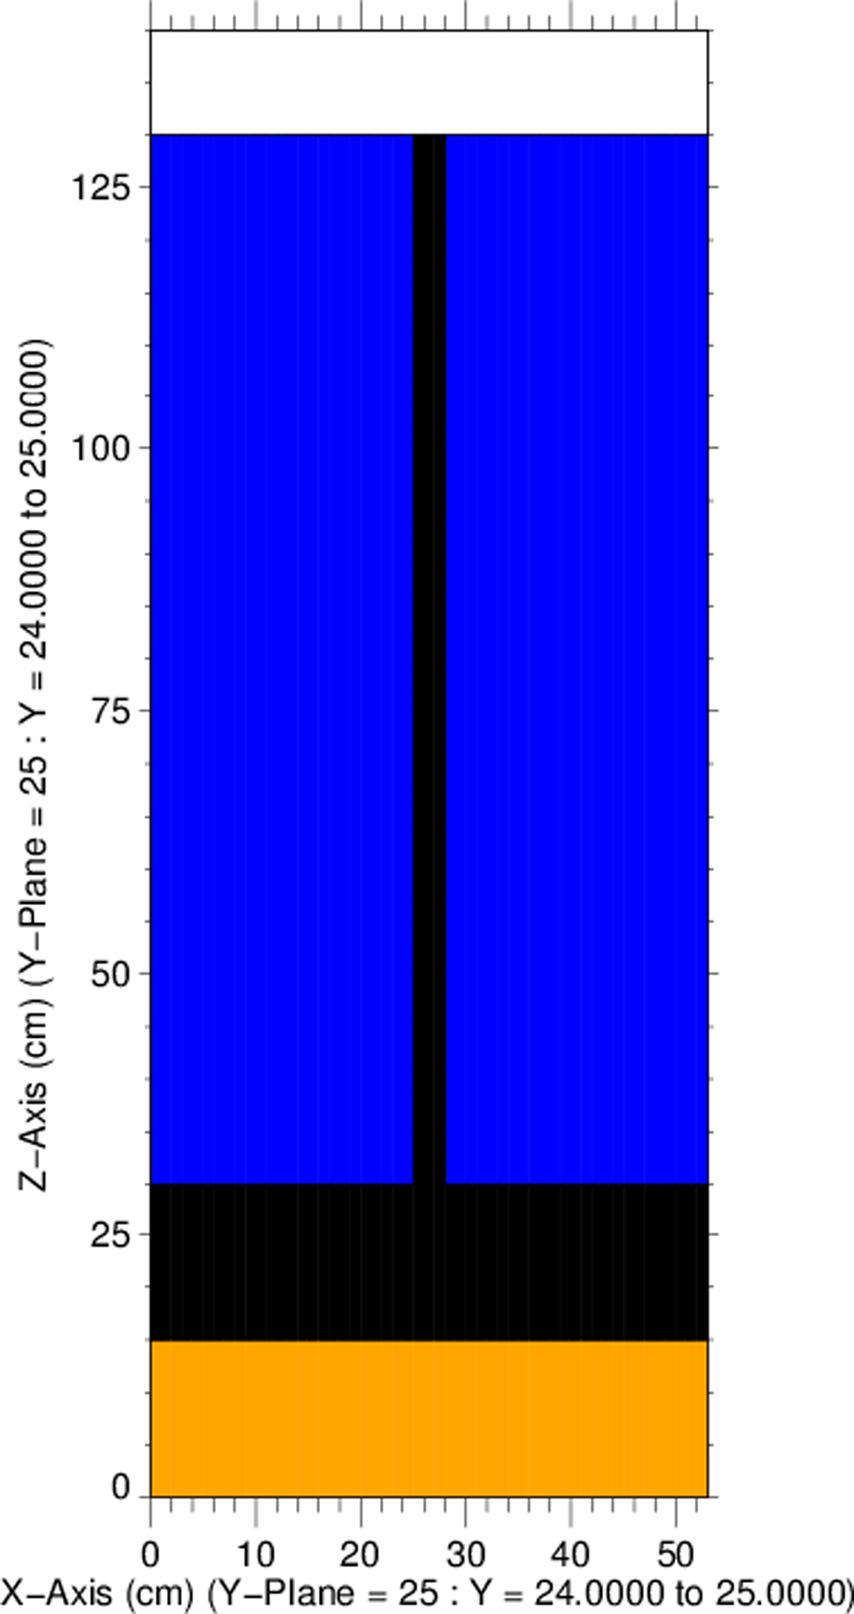
\includegraphics[width=0.4\textwidth]{img/steel-xz.png}
\caption{Steel plate in water geometry ($x-z$ slice through $y = 25$ cm) 
         \cite{wilsonslaybaugh}.}
\label{steelxz}
\end{figure}

The problem measurements are $53\times50\times140$ cm. The scenario is uniform 
in the $y$-direction and materials vary mainly in the $z$-direction. The source
region extends from 0 to 15 cm, the steel shield extends between 15 and 30 cm, 
the water and steel plate extend from 30 to 130 cm, and the air extends from 
130 to 140 cm. The steel plate is 3 cm wide and is centered at $x = 26.5$ cm. 
Vacuum boundary conditions were used at the problem boundaries.

A non-uniform Cartesian mesh was used for the spatial discretization in the 
deterministic calculations. In the $x$-direction, voxel width is 5 cm between
$x = 0$ cm and $x = 25$ cm, 0.5 cm between $x = 25$ cm and $x = 28$ cm, and 5 
cm between $x = 28$ cm and $x = 53$ cm. A uniform spacing of voxel width 1 cm 
was used in the $y$-direction. In the $z$-direction, the spatial cell width is
3 cm between $z = 0$ cm and $z = 30$ cm and 2 cm between $z = 30$ cm and 
$z = 140$ cm.

\begin{table}[!htb]
\centering
\caption{Materials and compositions in the steel plate in water scenario.}
\label{steel-mat}
\begin{tabular}{l|cc}
Material & \multicolumn{2}{c}{Isotopes (Atomic \%)} \\ \hline
\multirow{5}{*}{Source}   & U-235   & (0.000247) \\
                          & U-238   & (0.009287) \\
                          & Zr-nat. & (0.004009) \\
                          & H-1     & (0.037394) \\
                          & O-16    & (0.034927) \\ \hline
\multirow{4}{*}{Air}      & N-14    & (0.784431) \\
                          & O-16    & (0.210748) \\
                          & Ar-nat. & (0.004671) \\
                          & C-nat.  & (0.000150) \\ \hline
\multirow{2}{*}{Carbon Steel} & C-nat.  & (0.022831) \\
                              & Fe-nat. & (0.977169) \\ \hline
\multirow{2}{*}{Water}        & H-1     & (2)        \\
                              & O-16    & (1)        \\
\end{tabular}
\end{table}

The composition of the neutron source block is a homogenization of water,
zirconium, and uranium and was calculated based on the geometry and composition
of the Rowlands UO$_2$ pin cell benchmark specification \cite{pincell}. The
source is a U-235 fission 
spectrum that is uniformly distributed throughout the homogenized material. The
compositions of air, carbon steel, and water were taken from the Compendium of 
Material Composition Data for Radiation Transport Modeling \cite{pnnl}.

%%---------------------------------------------------------------------------%%
\subsection{Dog-Legged Void Neutron}

The next problem modeled is the dog-legged void neutron (DLVN) experimental 
benchmark, which was designed to measure neutron streaming in iron with air
voids. The model used in the following calculations was constructed from
References \cite{sw-dlvn,j-dlvn,dlvn1991}. The two materials used in the
problem are elemental iron and polyethylene. The polyethylene composition used
was C$_2$H$_4$. This is listed as ``polyethylene, non-borated'' and is material
248 in Reference \cite{pnnl}. 

\begin{figure}[!htb]
\centering
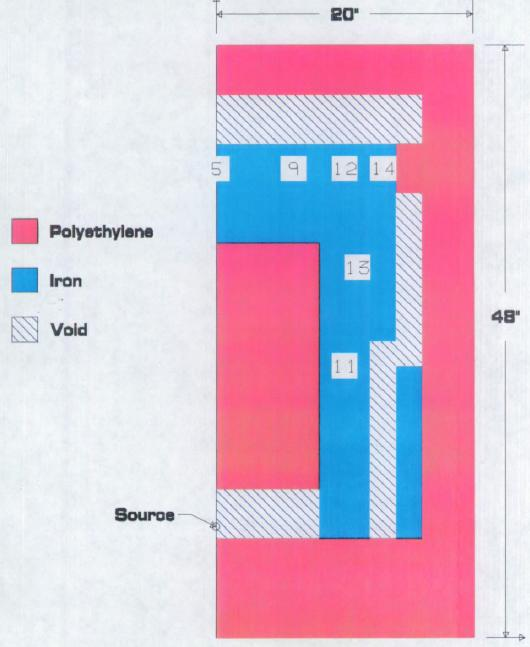
\includegraphics[width=0.5\textwidth]{img/dlvn.png}
\caption{Centerline cutaway of DLVN setup \cite{sw-dlvn}.}
\label{dlvn}
\end{figure}

The problem measurements are $40\times54\times48$ inches. A uniform spatial
mesh was imposed over the entire problem, with voxels measuring 1 inch per side.
The neutron source in this problem is a Cf-252 point source located at the 
center of the $x-$ and $y-$directions and at $z = 9$ inches.
This point source was approximated as a small volumetric source in the tests in
this work.

The experimental configuration is symmetric about the $y-z$ plane at $x = 0$
and so is usually simulated with a reflecting boundary at $x = 0$ and vacuum
boundaries on all other sides of the configuration. For the tests in this work,
the use of reflecting boundary conditions was not available, so the model used 
was constructed to represent the entire experimental geometry configuration.
Vacuum boundary conditions were applied to the outside of the entire problem.

%%---------------------------------------------------------------------------%%
\subsection{Calculation Parameters}

All of the deterministic calculations used 32 processes on a 2.8GHz AMD 
Opteron\texttrademark\ 6320 Processor \cite{amd}, two for each logical CPU
unit. With this in mind, all deterministic calculations were set to use the
same Denovo computational block structure of 8 blocks 
in the $x-$dimension, 4 blocks in the $y-$dimension, and 1 block in the 
$z-$dimension; thus the total number of computational blocks equals the number
of processes. Denovo uses the Koch-Baker-Alcouffe (KBA) parallel sweep
algorithm for high parallel efficiency in calculating transport sweeps
\cite{denovo}; the aforementioned block structure was chosen to achieve the
same parallel performance among all test case deterministic simulations. 

The two test cases use the same coarse energy group structure specified in 
the ``27n19g'' library; the groups in this library are listed in Table A-1 of
Appendix A of the ADVANTG technical report \cite{advantg}. Because 
energy discretization is treated the same way between the traditional discrete
ordinates formulation and the LDO equations, it was assumed that energy group 
structure would not greatly impact the comparative results.
The step characteristics (SC) spatial discretization was used in all of the
calculations and all runs used a P$_5$ scattering expansion.

For the comparisons presented here, quadrature sets of similar angular mesh
refinement were chosen such that the quadrature sets have approximately the 
same total number of angles, with the exception of the Galerkin quadrature set.
The QR quadrature set is of order 4 and has 128 angles, the LDFE set is order 1
with 128 angles, and the LDO set is of order 11 with 144 angles. 
The Galerkin quadrature set chosen as the representative example here is of
order 4 and has 24 angles. This set was chosen because its corresponding \pn\
order is 5 and so the scattering data used matches that of the other quadrature
types. At the time of this writing, Galerkin quadrature sets are implemented in
the Exnihilo framework with the restriction that the \pn\ order be one greater
than the \sn\ order.

%---------------------------------------------------------------------------%%
\section{Results}
\label{sec:results}

\subsection{Steel Plate Embedded in Water}

\subsection{Dog-Legged Void Neutron}

\subsection{Summary}

%---------------------------------------------------------------------------%%
\section{Conclusions and Future Work}
\label{sec:conclusions}

In this work we have seen that the LDO equations' scalar flux solutions are
comparable to those of standard quadrature types. Of particular interest is
the proximity of the LDO solutions to the QR solutions.

\pagebreak
\section*{Acknowledgments}

This material is based upon work supported under an Integrated
University Program Graduate Fellowship as well as supported by the Department 
of Energy under Award Number(s) DE-NE0008661. This report was prepared as an
account of work sponsored by an agency of the United States Government.
Neither the United States Government nor any agency thereof, nor any of their
employees, makes any warranty, express or limited, or assumes any legal
liability or responsibility for the accuracy, completeness, or usefulness of
any information, apparatus, product, or process disclosed, or represents that
its use would not infringe privately owned rights. Reference herein to any 
specific commercial product, process, or service by trade name, trademark, 
manufacturer, or otherwise does not necessarily constitute or imply its 
endorsement, recommendation, or favoring by the United States Government or
any agency thereof. The views and opinions of authors expressed herein do not 
necessarily state or reflect those of the United States Government or any 
agency thereof.

\pagebreak

\bibliographystyle{nse}
\bibliography{ldo-deterministic}

\end{document}

